%%%%%%%%%%%%%%%%%%%%%%%%%%%%%%%%%%%%%%%%%
% Beamer Presentation
% LaTeX Template
% Version 1.0 (10/11/12)
%
% This template has been downloaded from:
% http://www.LaTeXTemplates.com
%
% License:
% CC BY-NC-SA 3.0 (http://creativecommons.org/licenses/by-nc-sa/3.0/)
%
%%%%%%%%%%%%%%%%%%%%%%%%%%%%%%%%%%%%%%%%%

%----------------------------------------------------------------------------------------
% PACKAGES AND THEMES
%----------------------------------------------------------------------------------------

\documentclass[table, xcolor={dvipsnames}, 9pt]{beamer}
\usepackage{tikz}
\usetikzlibrary{positioning}
\mode<presentation> {

% The Beamer class comes with a number of default slide themes
% which change the colors and layouts of slides. Below this is a list
% of all the themes, uncomment each in turn to see what they look like.

%\usetheme{default}
%\usetheme{AnnArbor}
%\usetheme{Antibes}
%\usetheme{Bergen}
%\usetheme{Berkeley}
%\usetheme{Berlin}
%\usetheme{Boadilla}
%\usetheme{CambridgeUS}
%\usetheme{Copenhagen}
%\usetheme{Darmstadt}
%\usetheme{Dresden}
%\usetheme{Frankfurt}
%\usetheme{Goettingen}
%\usetheme{Hannover}
%\usetheme{Ilmenau}
%\usetheme{JuanLesPins}
%\usetheme{Luebeck}
% \usetheme{Madrid}
\usetheme{metropolis}
%\usetheme{Malmoe}
%\usetheme{Marburg}
%\usetheme{Montpellier}
%\usetheme{PaloAlto}
%\usetheme{Pittsburgh}
%\usetheme{Rochester}
%\usetheme{Singapore}
%\usetheme{Szeged}
%\usetheme{Warsaw}

% As well as themes, the Beamer class has a number of color themes
% for any slide theme. Uncomment each of these in turn to see how it
% changes the colors of your current slide theme.

%\usecolortheme{albatross}
%\usecolortheme{beaver}
%\usecolortheme{beetle}
%\usecolortheme{crane}
%\usecolortheme{dolphin}
%\usecolortheme{dove}
%\usecolortheme{fly}
%\usecolortheme{lily}
%\usecolortheme{orchid}
%\usecolortheme{rose}
%\usecolortheme{seagull}
%\usecolortheme{seahorse}
%\usecolortheme{whale}
%\usecolortheme{wolverine}

%\setbeamertemplate{footline} % To remove the footer line in all slides uncomment this line
%\setbeamertemplate{footline}[page number] % To replace the footer line in all slides with a simple slide count uncomment this line

%\setbeamertemplate{navigation symbols}{} % To remove the navigation symbols from the bottom of all slides uncomment this line
}
\setbeamertemplate{footline}{}
\addtobeamertemplate{footnote}{}{\vspace{24pt}}
\usepackage{graphicx} % Allows including images
\usepackage{booktabs} % Allows the use of \toprule, \midrule and \bottomrule in tables
\usepackage{multirow}
\usepackage{natbib}
\usepackage[]{hyperref}
\usepackage{diagbox}
\usepackage{makecell}
\usepackage{subfig}
\usepackage{amsmath}
\usepackage{amsfonts,amsthm,amsmath,amssymb}    
\usepackage{bbm}
\usepackage{bm}
\usepackage{empheq}
\makeatletter
\let\save@measuring@true\measuring@true
\def\measuring@true{%
  \save@measuring@true
  \def\beamer@sortzero##1{\beamer@ifnextcharospec{\beamer@sortzeroread{##1}}{}}%
  \def\beamer@sortzeroread##1<##2>{}%
  \def\beamer@finalnospec{}%
}
\makeatother
\hypersetup{unicode=true,
            pdfusetitle,
            bookmarks=true,
            bookmarksnumbered=true,
            bookmarksopen=true,
            bookmarksopenlevel=2,
            breaklinks=false,
            pdfborder={0 0 1},
            backref=true,
            hypertexnames=false,
            pdfstartview={XYZ null null 1}}
\usepackage{xcolor}
\newcommand\myheading[1]{%
  \par\bigskip
  {\Large\bfseries#1}\par\smallskip}
\newcommand\given[1][]{\:#1\vert\:}
\theoremstyle{newstyle}
\newtheorem{thm}{Theorem}
\newtheorem{prop}[thm]{Proposition}
\newtheorem{lem}{Lemma}
\newtheorem{cor}{Corollary}
\newtheorem{defin}{Definition}
\newcommand*\diff{\mathop{}\!\mathrm{d}}
\newcommand*\Diff[1]{\mathop{}\!\mathrm{d^#1}}
\newcommand*{\QEDA}{\hfill\ensuremath{\blacksquare}}%
\newcommand*{\QEDB}{\hfill\ensuremath{\square}}%
\DeclareMathOperator{\E}{\mathrm{E}}
\DeclareMathOperator{\R}{\mathbb{R}}
\DeclareMathOperator{\Var}{\rm{Var}}
\DeclareMathOperator{\Cov}{\rm{Cov}}
\DeclareMathOperator{\e}{\rm{e}}
\DeclareMathOperator{\logit}{\rm{logit}}
\DeclareMathOperator{\indep}{{\perp\!\!\!\perp}}
%\DeclareMathOperator{\Pr}{\rm{Pr}}
\newenvironment{Column}[1][.5\linewidth]{\begin{column}{#1}}{\end{column}}
%----------------------------------------------------------------------------------------
% TITLE PAGE
%----------------------------------------------------------------------------------------

\title[]{Sensitivity analysis} % The short title appears at the bottom of every slide, the full title is only on the title page

\author{Thomas Leavitt} % Your name
\institute[] % Your institution as it will appear on the bottom of every slide, may be shorthand to save space
{
% Your institution for the title page
\medskip
\textit{} % Your email address
}
\date{\today} % Date, can be changed to a custom date

\begin{document}

\begin{frame}
\titlepage % Print the title page as the first slide
\end{frame}

%\begin{frame}
%\frametitle{Overview} % Table of contents slide, comment this block out to remove it
%\tableofcontents % Throughout your presentation, if you choose to use \section{} and \subsection{} commands, these will automatically be printed on this slide as an overview of your presentation
%\end{frame}

%------------------------------------------------------------------------
% PRESENTATION SLIDES
%------------------------------------------------------------------------
\section{A model for sensitivity analysis}
\begin{frame}{Sensitivity analysis model}
\begin{itemize}
\item The model of an observational study states that units are individually assigned to treatment or control by $n$ \textit{independent}, but not necessarily \textit{identically distributed}, coin tosses: \pause
\begin{itemize}
\item $Z_i \sim \pi_i^{z_i} \left(1 - \pi_i\right)^{1 - z_i}, i = 1, \dots n$, where $\pi_i \in (0, 1)$ for all $i$
\end{itemize}
\item \pause Consider the following model for the distribution of treatment assignments: \pause
\begin{align*} 
\Pr\left(\mathbf{Z} = \mathbf{z}\right) & = \prod \limits_{i = 1}^n \lambda\left(\mathbf{x}_i, u_i\right)^{z_i} \left(1 - \lambda\left(\mathbf{x}_i, u_i\right)\right)^{1 - z_i}, \\
\text{where } \lambda\left(\mathbf{x}_i, u_i\right) & = \cfrac{\exp\left(\bm{x}_i\bm{\beta} + \gamma u_i\right)}{1 + \exp\left(\bm{x}_i\bm{\beta} + \gamma u_i\right)}.
\end{align*}
\end{itemize}
\end{frame}
%------------------------------------------------------------------------
\begin{frame}{Conditioning on a sufficient statistic}
\begin{itemize}
\item In general, there are $2^n$ possible assignments
\item \pause But we condition on the number of treated units, $n_1 = \sum \limits_{i = 1}^n Z_i$, which is sufficient to eliminate the parameter(s) $\bm{\beta}$ under perfect balance within strata:
\begin{itemize}
\item \pause Assume that $\bm{x}_i = \bm{x}_j$ for all units $i$ and $j \neq i$ in the same stratum
\item \pause Then conditioning on a sufficient statistic yields the distribution
\begin{align*}
\Pr\left(\mathbf{Z} = \mathbf{z} | n_1\right) & = \cfrac{\exp\left(\gamma \mathbf{z}^t\mathbf{u}\right)}{\sum \limits_{\mathbf{b} \in \Omega}\exp\left(\gamma \mathbf{b}^t\mathbf{u}\right)},
\end{align*}
where the superscript $t$ denotes matrix transposition
\item \pause See example in \texttt{R} ...
\end{itemize}
\item \pause Under assumed logit model, distribution on $\Omega = \left\{\bm{z}: \sum_{i = 1}^n z_i = n_1\right\}$ determined solely by $\gamma$ and $\mathbf{u}$
\end{itemize}
\end{frame}
%------------------------------------------------------------------------
\begin{frame}{Unobserved confounding}
\begin{itemize}
\item Express unobserved confounding in terms of a scalar $u_i \in \left[0, 1\right]$
\item \pause There is always an unobserved confounder of this form such that strong ignorability would hold if we had access to this confounder \citep[][300, footnote 33]{rosenbaum2017}: \pause 
\end{itemize}
\begin{figure}
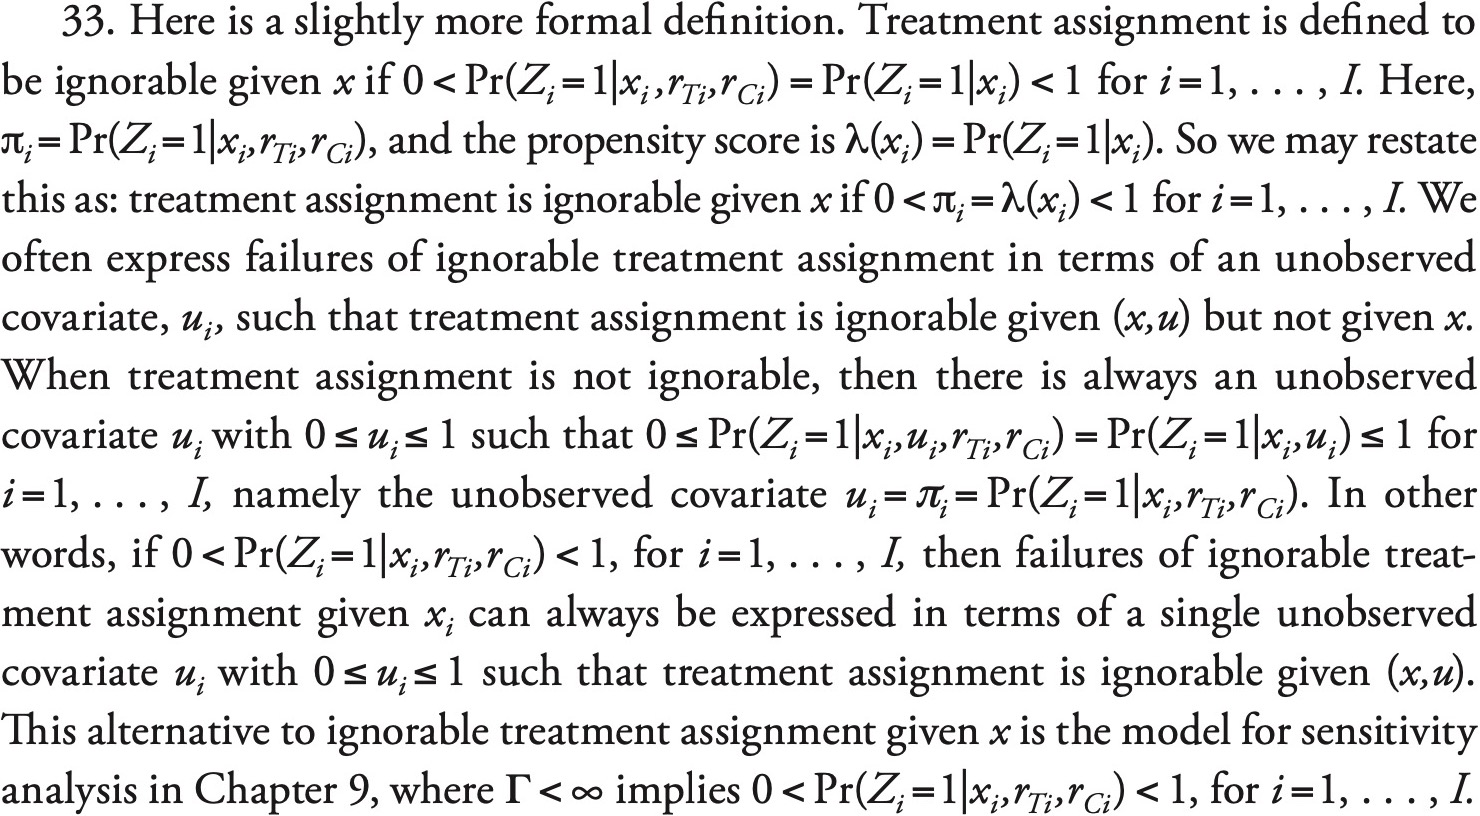
\includegraphics[width = \linewidth]{Rosenbaum_2017_page_300_footnote_33.jpg}
\end{figure}
\end{frame}
%------------------------------------------------------------------------
\section{Conservative sensitivity analysis without strata}
\begin{frame}{Conservative sensitivity analysis}
\begin{itemize}
\item For a fixed $\gamma \geq 0$, find $\mathbf{u}$ that maximizes the p-value 
\begin{itemize}
\item \pause I.e., find $\max \limits_{\mathbf{u} \in \mathcal{U}} \Pr\left(t\left(\mathbf{Z}, \mathbf{y}\right) \geq k \right)$, where you replace $k$ with the observed test statistic $t\left(\mathbf{Z}, \mathbf{Y}\right)$
\end{itemize}	
\item \pause \citet{rosenbaumkrieger1990} show that, for a large class of test statistics, the following result holds:
\begin{itemize}
\item[] 
\pause Renumber the subjects such that $y_1 \geq y_2 \geq \ldots \geq y_n$. The $\mathbf{u} \in \mathcal{U}$ that maximizes the p-value is some $\mathbf{u} \in \mathcal{U}^+ \subset \mathcal{U} = \left[0, 1\right]^n$, where
\begin{align*}
\mathcal{U}^+ & = \left\{
\begin{bmatrix} 1 \\ 0 \\ 0 \\ \vdots \\ 0 \end{bmatrix},
\begin{bmatrix} 1 \\ 1 \\ 0 \\ \vdots \\ 0 \end{bmatrix},
\ldots , 
\begin{bmatrix} 1 \\ 1 \\ \vdots \\ 1 \\ 0 \end{bmatrix}
\right\}
\end{align*}
\end{itemize}
\item \pause All $\mathbf{u} \in \mathcal{U}^+$ have at least one $1$ and one $0$ and the $1$s all appear in the coordinates corresponding to the largest 
\end{itemize}
\end{frame}
%------------------------------------------------------------------------
\section{Conservative sensitivity analysis with strata}
\begin{frame}{Conservative sensitivity analysis in stratified studies}
\begin{itemize}
\item Let the index $s \in \left\{1, \ldots, S\right\}$ runs over the $S$ strata
\item \pause Then order the $n$ units lexically by stratum and then in decreasing order within strata by the value of the outcome $y_{is}$.
\begin{itemize}
\item \pause E.g., in \texttt{R}: \texttt{data <- dplyr::arrange(.data = data, strata, desc(y))}
\end{itemize}	
\item \pause The worst-case $\mathbf{u} \in \mathcal{U}^+$ cannot be found by finding $\mathbf{u}_s \in \mathcal{U}_s^+$ in each stratum one at a time
\item \pause All $n$ coordinates of $\mathbf{u} \in \mathcal{U}^+$ must be found simultaneously
\item \pause Hence, there are $\prod \limits_{s = 1}^S \left(n_s - 1\right)$ candidate values to consider
\begin{itemize}
\item \pause Usually computationally intractable, even in relatively small studies
\end{itemize}
\end{itemize}
\end{frame}
%------------------------------------------------------------------------
\begin{frame}{Approximate worst-case sensitivity analysis}
\begin{itemize}
\item Consider the test statistic of $t\left(\mathbf{Z}, \mathbf{y}\right) = \mathbf{Z}^t\mathbf{q} = \sum \limits_{s = 1}^S \sum \limits_{i = 1}^{n_s} Z_{si} q_{si}$, where $\mathbf{y}$ denotes that the sharp null is true and $\mathbf{q} = \mathbf{q}\left(\mathbf{y}\right)$ is a pre-specified function of the outcome vector $\mathbf{y}$
\item \pause The use of sum statistics has the benefit of being easily coupled with finite population central limit theorems \citep[see][]{liding2017}
\item \pause Roughly speaking, $\cfrac{\mathbf{Z}^t\mathbf{q} - \E\left[\mathbf{Z}^t \mathbf{q}\right]}{\Var\left[\mathbf{Z}^t\mathbf{q} \right]^{1/2}}$ converges in law to a standard Normal distribution as $S \to \infty$ with $1 \leq n_{1,s} < n_s \leq \tilde{n}$ for some bound $\tilde{n}$ \citep[see][]{gastwirthetal2000}
\item \pause We can use an asymptotic approximation to the solution of $\max \limits_{\mathbf{u} \in \mathcal{U}^+} \Pr\left(t\left(\mathbf{Z}, \mathbf{y}\right) \geq k \right)$ 
\begin{itemize}
\item \pause We don't need to consider all of the $\left\lvert\mathcal{U}^+\right\rvert$ candidate values of $\mathbf{u}$
\end{itemize}
\end{itemize}
\end{frame}
%------------------------------------------------------------------------
\begin{frame}{Approximate worst-case sensitivity analysis}
\begin{itemize}
\item The logic of the asymptotically separable algorithm \citep{gastwirthetal2000} is as follows:
\begin{enumerate}
\item \pause For sum statistics, we have closed form expressions for their expectations and variances under any forms of confounding
\item \pause Therefore, for a fixed $\gamma \geq 0$, find the values of $\mathbf{u} \in \mathcal{U}^+$ that maximize the expectation of the null sum statistic under the sharp null
\item \pause Among the values of $\mathbf{u} \in \mathcal{U}^+$ that maximize the expectation, choose the $\mathbf{u} \in \mathcal{U}^+$ that maximizes the variance
\end{enumerate}	
\item \pause \citet{gastwirthetal2000} call this approach an asymptotically separable approximation because it allows the optimization algorithm to be done in each stratum individually
\item \pause This algorithm does not necessarily find $\max \limits_{\mathbf{u} \in \mathcal{U}} \Pr\left(t\left(\mathbf{Z}, \mathbf{y}\right) \geq k \right)$
\begin{itemize}
\item \pause But, as $S \to \infty$ with $1 \leq m_s < n_s \leq \tilde{n}$, the difference between $\max \limits_{\mathbf{u} \in \mathcal{U}} \Pr\left(t\left(\mathbf{Z}, \mathbf{y}\right) \geq k \right)$ and $\mathbf{u}$ returned by the algorithm is negligible
\end{itemize}
\end{itemize}
\end{frame}
%------------------------------------------------------------------------
\begin{frame}{An alternative simulation-based sensitivity analysis}
\begin{itemize}
\item In many actual studies, the asymptotically separable approximation may be poor
\item \pause Scholars are often interested in test statistics other than sum statistics, e.g., energy test statistics \citep{szekelyrizzo2013,rizzoszekely2016,szekelyrizzo2017}
\item \pause Instead, randomly sample from $\mathcal{U}^+$ and, for a given $\gamma \geq 0$, choose the sampled $\mathbf{u}$ that maximizes the p-value
\end{itemize}
\end{frame}
%------------------------------------------------------------------------
\section{Comparison of asymptotically separable and simulation-based approximations}
\begin{frame}{An alternative simulation-based sensitivity analysis}
\begin{itemize}
\item Consider the following simple example:
\begin{table}
\centering
    \begin{tabular}{l|l}
    $\mathbf{z}$ & $\mathbf{y}$ \\ \midrule
    0 & 11 \\
    1 & 20  \\
    0 & 5  \\
    1 & 15 \\
    $\vdots$ & $\vdots$ \\ 
    0 & 15  \\
    1 & 37 \\
    \end{tabular}
\end{table}
\item[]
\item \pause There are only 20 units, so we can easily compare exact, simulation-based and asymptotically separable sensitivity analyses
\end{itemize}
\end{frame}
%------------------------------------------------------------------------
\begin{frame}{Sensitivity analysis}
\begin{figure}
\includegraphics[width = 0.9\linewidth]{sens_plot.pdf}
\caption{The dotted line is the asymptotically separable approximation, the solid line is the exact sensitivity analysis and the dashed line is the simulation-based sensitivity analysis}
\end{figure}
\end{frame}
%------------------------------------------------------------------------
\begin{frame}{Comparison of asymptotically separable and simulation-based approximations}
\begin{itemize}
\item Consider two different studies:
\begin{enumerate}
\item \pause A regression discontinuity design without strata on incumbency advantage in close US House of Representatives races from 1942--2008 \citep{caugheysekhon2011}
\item \pause A matching design on whether UN interventions cause peace \citep{gilligansergenti2008}
\end{enumerate}	
\end{itemize}	
\end{frame}
%------------------------------------------------------------------------
\begin{frame}{Sensitivity analysis in RDD}
\begin{figure}
\includegraphics[width = \linewidth]{rdd_sens_plot.pdf}
\caption{The dotted line is the asymptotically separable approximation, the dashed line is the simulation-based sensitivity analysis}
\end{figure}
\end{frame}
%------------------------------------------------------------------------
\begin{frame}{Sensitivity analysis in matched design}

\begin{figure}
\includegraphics[width = \linewidth]{match_sens_plot.pdf}
\caption{The dotted line is the asymptotically separable approximation, the dashed line is the simulation-based sensitivity analysis}
\end{figure}

\end{frame}
%------------------------------------------------------------------------

\begin{frame}[allowframebreaks]
\frametitle{References} 
\scriptsize
\bibliographystyle{chicago}
\bibliography{../../BIB/Master_Bibliography}   % name your BibTeX data base
\end{frame}
%------------------------------------------------------------------------
\end{document}
